
\begin{figure}[H]
	\centering
	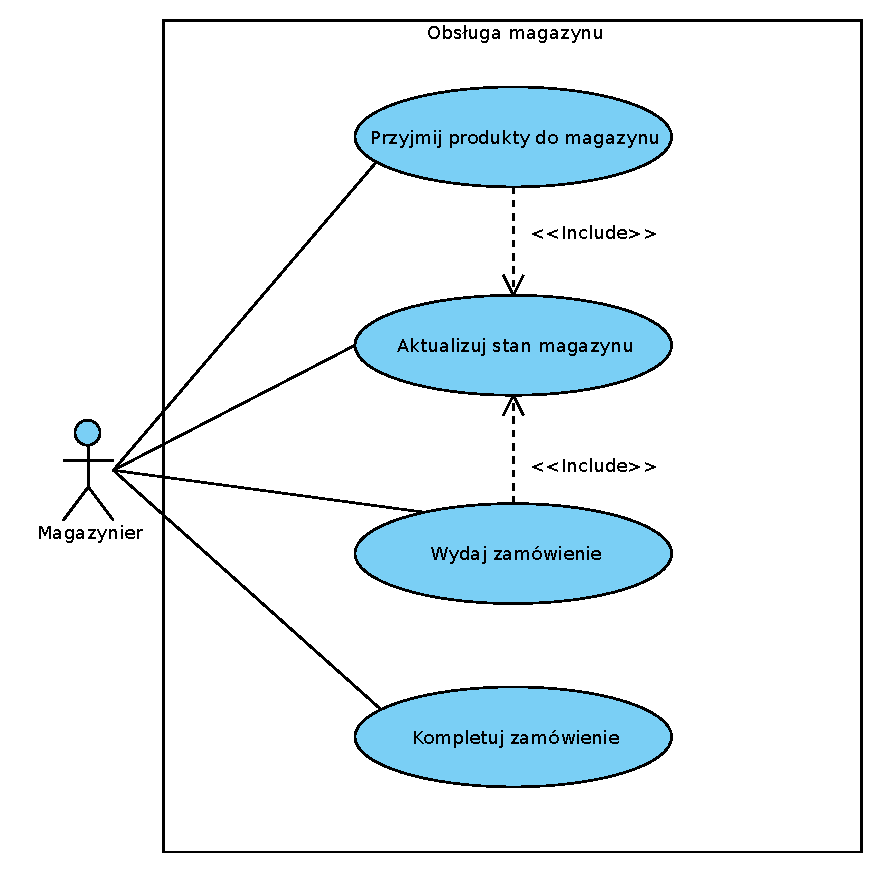
\includegraphics[width=.8\textwidth]{img/UC/magazyn.eps}
\end{figure}

\textbf{Numer i Nazwa przypadku użycia:} UC01 - Przyjmij produkty do magazynu \\
\textbf{Autor:} Magazynier\\
\textbf{Cel przypadku użycia:} Dodanie produktów recyklingu do magazynu i aktualizacja stanu magazynu \\
\textbf{Kontekst użycia:} przechowanie produktów recyklingu w magazynie\\
\textbf{Zakres:} system magazynowy \\
\textbf{Poziom:} biznesowy \\
\textbf{Aktor główny:} Magazynier \\
\textbf{Uczestnicy:} Kierowca \\
\textbf{Wyzwalacz:} dostarczenie przez kierowce produktów do magazynu \\
\textbf{Warunek początkowy:} kierowca ma produkty recyklingu, które należy zmagazynować oraz ich listę \\
\textbf{Minimalna gwarancja:} w przypadku, gdy produkty nie zostaną zmagazynowane, stan magazynu nie będzie zmieniany \\
\textbf{Główny scenariusz powodzenia:} \\
	\begin{enumerate}
		\item Kierowca przywozi produkty
		\item Magazynier układa je w magazynie
		\item Magazynier aktualizuje stan magazynu
	\end{enumerate}

\textbf{Numer i Nazwa przypadku użycia:} UC02 - Wydaj zamówienie \\
\textbf{Autor:} Magazynier\\
\textbf{Cel przypadku użycia:} Wydanie kierowcy produktów, ujętych w zamówieniu \\
\textbf{Kontekst użycia:} potrzeba przetransporotowania produktów do kupca\\
\textbf{Zakres:} system magazynowy \\
\textbf{Poziom:} biznesowy \\
\textbf{Aktor główny:} Magazynier \\
\textbf{Uczestnicy:} Kierowca \\
\textbf{Wyzwalacz:} przyjazd kierowcy do magazynu \\
\textbf{Warunek początkowy:} kierowca ma zamówienie \\
\textbf{Minimalna gwarancja:} w przypadku, gdy nie można skompletować zamówienia stan magazynu się nie zmieni \\
\textbf{Główny scenariusz powodzenia:} 
	\begin{enumerate}
		\item Kierowca przekazuje numer zamówienia magazynierowi
		\item Magazynier wydaje produkty kierowcy
		\item Magazynier uaktualnia stan magazynu
	\end{enumerate}
\textbf{Rozszerzenia:} \\
1.1 W przypadku gdy magazynier nie otrzymał wcześniej informacji o zamówieniu, kompletuje je teraz, w razie niepowodzenia produkty nie zostają wydane\\

\textbf{Numer i Nazwa przypadku użycia:} UC03 - Aktualizuj stan magazynu \\
\textbf{Autor:} Magazynier\\
\textbf{Cel przypadku użycia:} Aktualizacja danych o stanie magayznu \\
\textbf{Kontekst użycia:} utrzymywanie aktualnej informacji o ilości produktów w magazynie \\
\textbf{Zakres:} system magazynowy \\
\textbf{Poziom:} użytkowy \\
\textbf{Aktor główny:} Magazynier \\
\textbf{Wyzwalacz:} wydanie lub przyjęcie produktów \\
\textbf{Warunek początkowy:} zmiana stanu magazynu \\
\textbf{Minimalna gwarancja:} w przypadku, gdy nie można zaktualizować stanu magazynu, jego stan pozostanie niezmieniony \\
\textbf{Główny scenariusz powodzenia:} 
	\begin{enumerate}
		\item Magazynier wpisuje informację o wydanych/przyjętych produktach
	\end{enumerate}

\textbf{Numer i Nazwa przypadku użycia:} UC04 - Kompletuj zamówienie \\
\textbf{Autor:} Magazynier\\
\textbf{Cel przypadku użycia:} Skompletowanie zamówienie w celu wydania go kierowcy \\
\textbf{Kontekst użycia:} chęć uporządkowania produktów do zamówienia w celu szybkiego ich przekazania kierowcy \\
\textbf{Zakres:} system magazynowy \\
\textbf{Poziom:} biznesowy \\
\textbf{Aktor główny:} Magazynier \\
\textbf{Wyzwalacz:} dostanie informacji o zamówieniu \\
\textbf{Warunek początkowy:} odpowiednia ilość towarów w magazynie \\
\textbf{Minimalna gwarancja:} w przypadku, gdy nie ma odpowiedniej ilości towarów w magazynie, zostanie wysłana informacja zwrotna  \\
\textbf{Główny scenariusz powodzenia:} 
	\begin{enumerate}
		\item Magazynier otrzymuje listę towarów, które wchodzą w skład zamówienia
		\item Magazynier sprawdza czy posiada ich odpowiednią ilość
		\item Magazynier przygotowuje zamówienie
	\end{enumerate}
\textbf{Rozszerzenia:} \\
2.1. Nie można skompletować zamówienia, zostaje wysłana informacja zwrotna o nieposiadanych towarach\\

\begin{figure}[H]
	\centering
	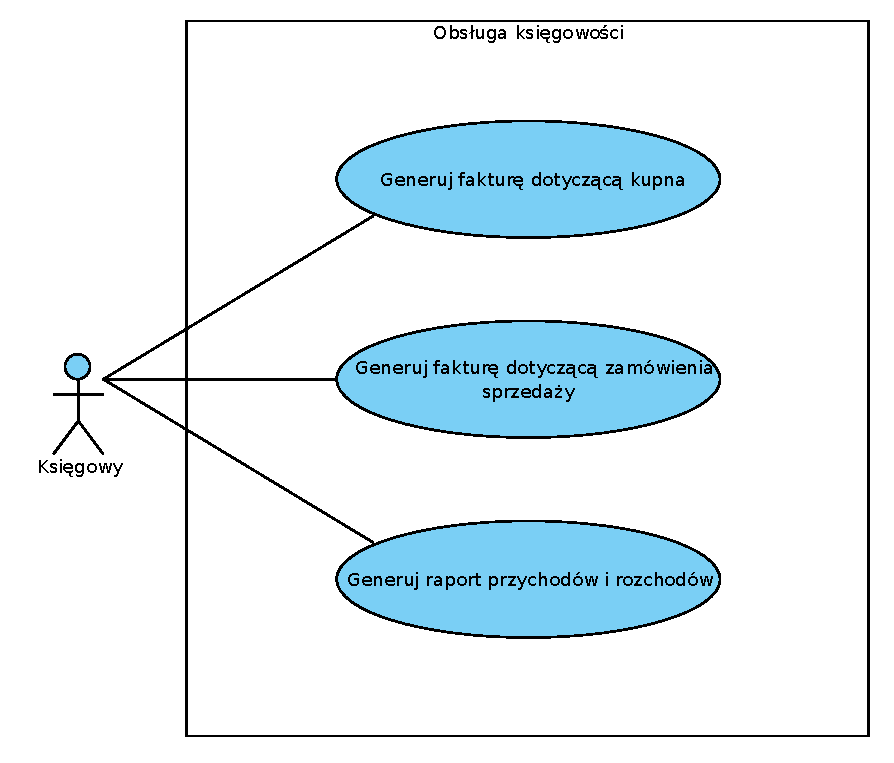
\includegraphics[width=.8\textwidth]{img/UC/ksiegowosc.eps}
\end{figure}

\textbf{Numer i Nazwa przypadku użycia:} UC05 - Generuj fakturę sprzedaży produktów recyklingu \\
\textbf{Autor:} Księgowy\\
\textbf{Cel przypadku użycia:} Wygnerowanie faktury \\
\textbf{Kontekst użycia:} otrzymanie dokumentu dowodu sprzedaży produktów  \\
\textbf{Zakres:} system księgujący \\
\textbf{Poziom:} biznesowy \\
\textbf{Aktor główny:} Księgowy \\
\textbf{Wyzwalacz:} sprzedaż produktów recyklingu \\
\textbf{Warunek początkowy:} księgowy posiada identyfikator zamówienia \\
\textbf{Minimalna gwarancja:} w przypadku, gdy nie będzie można wygenerować faktury, system poinformuje o tym aktora, nie generując błędnego dokumentu \\
\textbf{Główny scenariusz powodzenia:} 
	\begin{enumerate}
		\item Księgowy wpisuje identyfikator zamówienia
		\item System sprawdza czy w systemie jest zamówienie, o danym identyfikatorze
		\item System generuje fakturę 
	\end{enumerate}
\textbf{Rozszerzenia:} \\
2.1 Jeżeli identyfikator jest niepoprawny, system informuje o tym księgowego i prosi go o ponowne podanie tego parametru

\textbf{Numer i Nazwa przypadku użycia:} UC06 - Generuj fakturę dotyczącą usłiugi przejęcia obowiązku recyklingu \\
\textbf{Autor:} Księgowy\\
\textbf{Cel przypadku użycia:} Wygnerowanie faktury \\
\textbf{Kontekst użycia:} otrzymanie dokumentu dowodu zakupu oświadczenia  \\
\textbf{Zakres:} system księgujący \\
\textbf{Poziom:} biznesowy \\
\textbf{Aktor główny:} Księgowy \\
\textbf{Wyzwalacz:} kupno oświadczenia oddzysku \\
\textbf{Warunek początkowy:} księgowy posiada identyfikator danych dotyczących odpowiedniej oferty sprzedaży \\
\textbf{Minimalna gwarancja:} w przypadku, gdy nie będzie można wygenerować faktury, system poinformuje o tym aktora, nie generując błędnego dokumentu \\
\textbf{Główny scenariusz powodzenia:} 
	\begin{enumerate}
		\item Księgowy wpisuje identyfikator do oferty sprzedaży
		\item System sprawdza czy w systemie jest oferta, o danym identyfikatorze
		\item System generuje fakturę 
	\end{enumerate}
\textbf{Rozszerzenia:} \\
2.1 Jeżeli identyfikator jest niepoprawny, system informuje o tym księgowego i prosi go o ponowne podanie tego parametru

\textbf{Numer i Nazwa przypadku użycia:} UC07 - Wprowadź dane faktury kupna oświadzczenia o przetworzeniu odpadów \\
\textbf{Autor:} Księgowy\\
\textbf{Cel przypadku użycia:} Wpisanie do systemu danych o fakturze \\
\textbf{Kontekst użycia:} posiadanie w bazie wszystkich informacji o operacjach firmy\\
\textbf{Zakres:} system księgujący \\
\textbf{Poziom:} biznesowy \\
\textbf{Aktor główny:} Księgowy \\
\textbf{Wyzwalacz:} kupno oświadczenia oddzysku \\
\textbf{Warunek początkowy:} księgowy posiada dane o fakturze kupna oświadczenia o przetworzeniu odpadów \\
\textbf{Minimalna gwarancja:} w przypadku, gdy nie będzie można wproawdzić danych do bazy, nie zostanie ona zmodyfikowana \\
\textbf{Główny scenariusz powodzenia:} 
	\begin{enumerate}
		\item Księgowy wpisuje dane z faktury do systemu
		\item System sprawdza czy format poszczególnych danych jest prawidłowy
		\item System wprowadza dane do systemu
	\end{enumerate}
\textbf{Rozszerzenia:} \\
2.1 Jeżeli jakieś dane są niepoprawne, księgowy zostaje o tym poinformowany i musi wprowadzić je ponownie

\textbf{Numer i Nazwa przypadku użycia:} UC08 - Generuj raport przychodów i rozchodów \\
\textbf{Autor:} Księgowy\\
\textbf{Cel przypadku użycia:} Wygnerowanie raportu o zyskach i stratach firmy \\
\textbf{Kontekst użycia:} otrzymanie raportu dla właściciela  \\
\textbf{Zakres:} system księgujący \\
\textbf{Poziom:} biznesowy \\
\textbf{Aktor główny:} Właściciel \\
\textbf{Aktor uczestniczący:} Księgowy \\
\textbf{Wyzwalacz:} właściciel chce mieć informację o przychodach i rozchodach firmy w danym okresie czasowym \\
\textbf{Warunek początkowy:} podanie ram czasowych  \\
\textbf{Minimalna gwarancja:} w przypadku, gdy nie będzie można wygenerować raportu, system poinformuje o tym właściciela, nie generując błędnych informacji \\
\textbf{Główny scenariusz powodzenia:} 
	\begin{enumerate}
		\item Właściciel podaje ramy czasowe okresu, ktory go interesuje
		\item System wybiera tylko te faktury, które zawierają się w podanym przedziale czasowym
		\item System generuje raport
	\end{enumerate}
\textbf{Rozszerzenia:} \\
1.1 Ramy czasowe są błędne - conajmniej jedna z wartości jest w przyszłości, system wygeneruje błąd i poprosi o ich ponowne wpisanie


\begin{figure}[H]
	\centering
	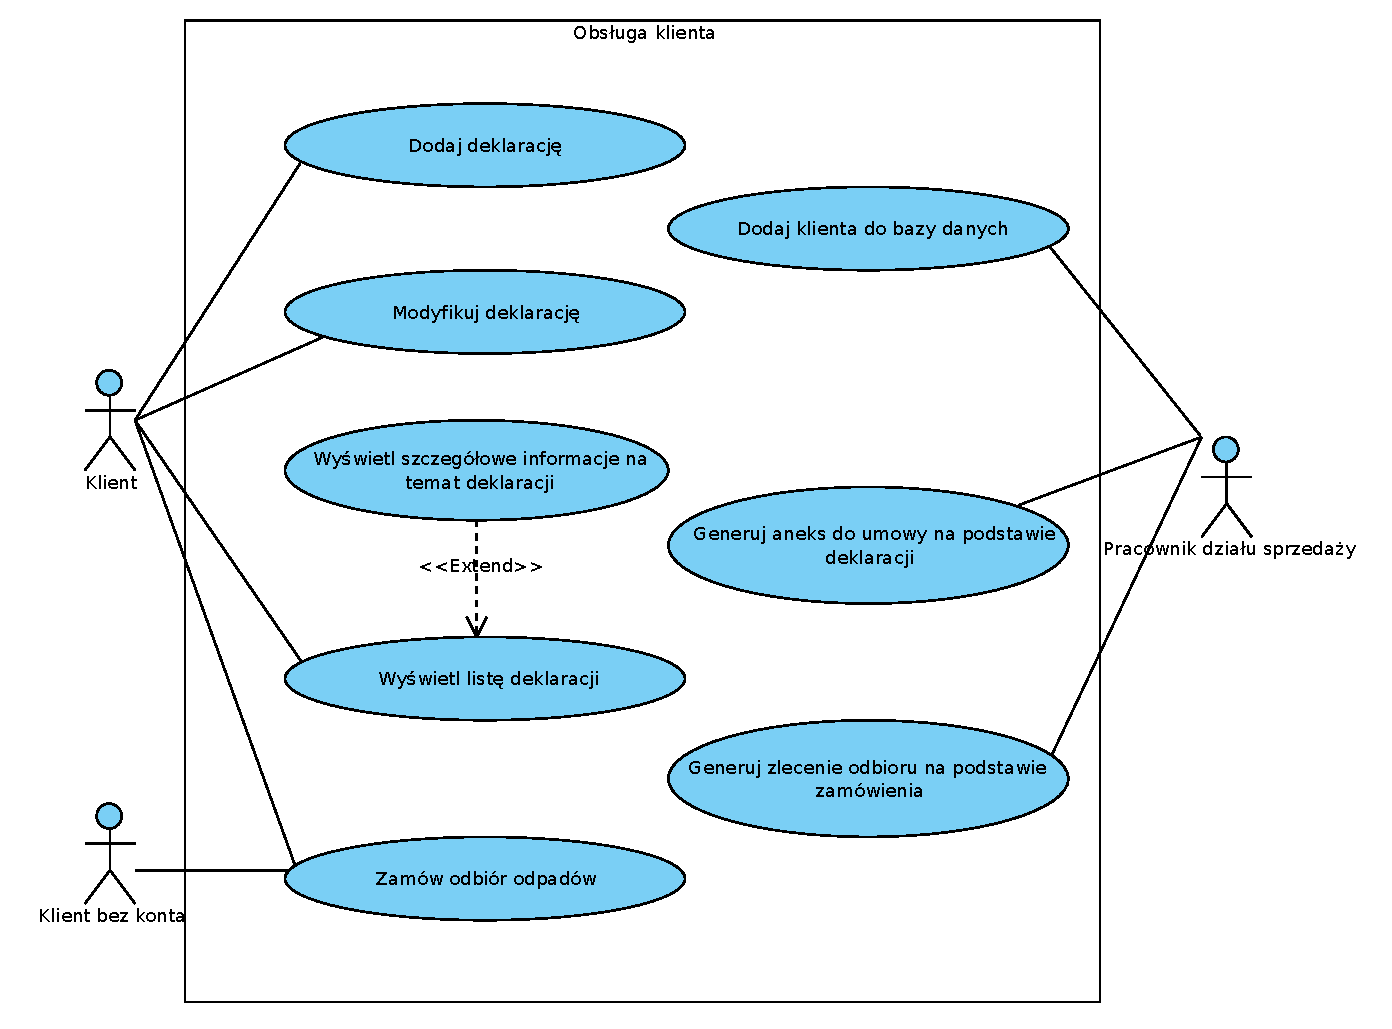
\includegraphics[width=1.1\textwidth]{img/UC/deklaracje.eps}
\end{figure}